
O processo de implementação do controlador utilizando a 
Lógica Paraconsistente Anotada Evidencial $E\tau$
produziu diversas tentativas, configurações, alterações, 
sendo que segue aquela que melhor resultado apresentou até
o devido ponto que se adotou nessa dissertação, 
não esgotando as formas e tentativas que poderão se seguir 
no decorrer da pesquisa.


\section{A proposição e a anotação}
Como ponto de partida, 
dado o sistema a ser controlado apresentado anteriormente, 
tendo como variável controlada 
a velocidade de rotação do disco acoplado ao eixo do motor e 
a variável manipilada o \emph{duty cycle} do sinal \emph{PWM} aplicado ao motor,
a proposição adotada então foi: 
"P: A velocidade de rotação é máxima."

Tal proposição permite que toda extensão de velocidades 
seja representa pelos Graus de evidência, 
sem que para uma dada velocidade de rotação ocorra que 
$Gct=0$ e $Gc = -0,5$,
onde mesmo não havendo contradição, 
a região de operação no reticulado não é o estado verdadeiro.

Os graus de evidência adotados são: 

\begin{itemize}
\item Grau de evidência favorável($\mu_0$): 
O valor de referência, ou seja, 
o valor desejado para a velocidade de rotação do sistema,
também chamado de \emph{setpoint}.
\item Grau de evidência favorável($\mu_1$): 
O valor lido pelo sensor de rotação, ou seja, a variável controlada.
Esse valor é convertido em 
Grau de evidência desfavorável($\lambda$),
para os devidos cálculos da LPA$E\tau$.
\end{itemize}

O diagrama da Figura \ref{fig:diagramaBlocosLPAEt} apresenta 
a planta do sistema $g(t)$ tendo como saída a 
variável controlada $c(t)$, 
velocidade de rotação do disco acoplado ao eixo do motor, 
e como entrada a variável manipulada $u(t)$, 
que é o parâmetro do \emph{PWM} 
que produz a sinal aplicado à planta.


\begin{figure}[!h]
\centering
\caption{Diagrama de blocos do controle utilizando a LPA$E\tau$}
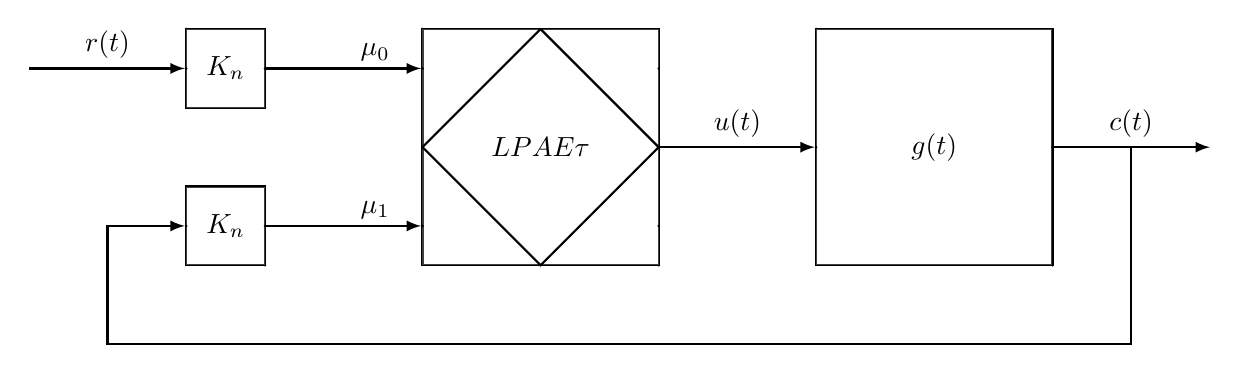
\begin{tikzpicture}[scale=1.0]
\tikzset{ >=latex, inner sep=0pt, outer sep=0pt,  }

%\draw [lightgray, dashed](0,0) grid (15,4.2);

%%% Blocos 

% Kn normalização rps -> 0..1
\node [fill=black, circle] (KSP0) at (2.0,4.0) { };
\node [fill=black, circle] (KSP1) at (3.0,3.0) { };
\draw[thick] (KSP0) rectangle (KSP1);
\fill[white, nearly transparent] (KSP0) rectangle (KSP1);
\node [fill=black, circle] (KSPin)  at (2.0,3.5) { }; 
\node [fill=black, circle] (KSPout) at (3.0,3.5) { }; 
\node (Kn1) at (2.5,3.5) {$K_n$};

% Kn Sensor
\node [fill=black, circle] (KS0) at (2.0,2.0) { };
\node [fill=black, circle] (KS1) at (3.0,1.0) { };
\draw[thick] (KS0) rectangle (KS1);
\fill[white, nearly transparent] (KS0) rectangle (KS1);
\node [fill=black, circle] (KSin)  at (2.0,1.5) { };
\node [fill=black, circle] (KSout) at (3.0,1.5) { };
\node (Kn2) at (2.5,1.5) {$K_n$};

% LPAEt
\node [fill=black, circle] (LPA0) at (5,4.0) { };
\node [fill=black, circle] (LPA1) at (8,1.0) { };
\draw[thick] (LPA0) rectangle (LPA1);
\fill[white, nearly transparent] (LPA0) rectangle (LPA1);
\draw [thick] (6.5,4.0) -- (8.0,2.5) -- (6.5,1.0) -- (5.0,2.5) -- (6.5,4.0);
\node (LPA2v) at (6.5,2.5) {$LPAE\tau$};
\node [fill=black, circle] (LPAu0)  at (5.0,3.5) { };
\node [fill=black, circle] (LPAu1)  at (5.0,1.5) { };
\node [fill=black, circle] (LPAgc)  at (8.0,3.5) { };
\node [fill=black, circle] (LPAs)   at (8.0,2.5) { };
\node [fill=black, circle] (LPAgct) at (8.0,1.5) { };
\node (LPA2vu0)  at (4.4,3.7) {$\mu _0$};
\node (LPA2vu1)  at (4.4,1.7) {$\mu _1$};

% Planta
\node [fill=black, circle] (GT0) at (10,4.0) { };
\node [fill=black, circle] (GT1) at (13,1.0) { };
\draw[thick] (GT0) rectangle (GT1);
\fill[white, nearly transparent] (GT0) rectangle (GT1);
\node [fill=black, circle] (GTin)  at (10.0,2.5) { };
\node [fill=black, circle] (GTout) at (13.0,2.5) { };
\node (planta) at (11.5,2.5) {$g(t)$};



%%% Linhas 

% set point
\draw [->, thick] (0.0,3.5) -- (KSPin);
\node (rt) at (1.0,3.8) {$r(t)$};

% GT -> fim
\draw [->, thick] (GTout) -- (15,2.5);
\node (ct) at (14.0,2.8) {$c(t)$};

% normalização 0..1 -> LPA2v u0
\draw [->, thick] (KSPout) -- (LPAu0);

% normalização 0..1 -> LPA2v u1
\draw [->, thick] (KSout) -- (LPAu1);

% LPAEt -> GT
\draw [->, thick] (LPAs) -- (GTin);
\node (ut) at (9.0,2.8) {$u(t)$};

% GT -> Kn Sensor
\draw [->, thick] (GTout) -- (14.0,2.5) -- (14.0,0.0) -- (1.0,0.0) -- (1.0,1.5) -- (KSin);


\end{tikzpicture}
\label{fig:diagramaBlocosLPAEt}

{\vspace{0.2cm} \small Fonte: Próprio autor}
\end{figure}


A variável manipulada $u(t)$ é produzida pelo 
bloco controlador $LPAE\tau$, 
e este recebe seus parâmetros no formato dos 
graus de evidência favoráveis $\mu_0$ ee $\mu_1$.
Sendo o parâmetro $\mu_1$ 
convertido internamente em $\lambda$ 
como grau de evidência desfavorável.

Os dois parâmetros que vão gerar os graus de evidência 
possuem a mesma natureza, a mesma escala, 
são a velocidade desejada e a velocidade lida pelo sensor,
de mode a poder comparar e utilizá-las nas operações da
LPA$E\tau$. 
Para adequação da escala das grandezas 
de referência $r(t)$ e da variável controlada $c(t)$
ao intervalo de trabalho dos parâmetros da LPA$E\tau$, 
é inserido um bloco de normalização do sinal em cada entrada.


Para a normalização os blocos $K_n$ realizam as seguinte operações:

\begin{equation}
\mu_0 = \frac{ r(t)}{c(t)_{\text{máx}}} \ \ \ \ \ \ \ \ \mu_1 = \frac{c(t)}{c(t)_{\text{máx}}}
\end{equation}

onde:

$c(t)_{\text{máx}}$: é a velocidade máxima produzida pelo sistema.





%%%%%%%%%%%%%%%%%%%%%%%%%%%%%%%%%%%%%%%%
%%%%%%%%%%%%%%%%%%%%%%%%%%%%%%%%%%%%%%%%
\newpage

\section{Ação de controle Liga-Desliga utilizando a LPA$E\tau$}

Assim como no capítulo sobre Ação de Controle, 
o tipo mais simples de controlador, o Liga-Desliga,
pode ser implementado utilizando a 
LPA$E\tau$, 
dividindo o reticulado conforme 
Figura \ref{fig:reticuladoEtOnOff}.

Utilizando o $Gct$ como variável condicionante:

\begin{itemize}
\item $Gct > 0 $: 
Para todas as combinaçãos de valores que produzam 
$\mu_0 > \mu_1$, 
ou seja, a variável de referência do sistema é 
maior do que a variável controlada,
o Grau de contradição encontra-se na condição de 
\textit{Inconsistência}, conforme exposto na Equação 
\ref{eq:grauInconsistenciaIndefinicao}.

Utilizando a Equação \ref{eq:grauContradicao} 
( $Gct = \mu + \lambda - 1 $ ) e 
substituindo 
$\mu$ por $\mu_0$ e $\lambda$ por $(1-\mu_1)$, 
temos:

\begin{equation}
Gct = \mu_0 + (1-\mu_1) -1
\end{equation}

simplificando temos então:

\begin{equation}
Gct = \mu_0 - \mu_1
\label{eq:gctmu0mu1}
\end{equation}

Supondo que o \emph{especialista 0} afirme que 
o valor da variável controlada é 25\% do valor máximo, 
o grau de evidência favorável 0 é $\mu_0 = 0,25$, 
enquanto que o \emph{especialista 1} afirma que 
seu valor é de 20\% do valor máximo, 
o grau de evidência favorável 1 é $\mu_1 = 0,20$. 
Substituindo $\mu_0$ e $\mu_1$ em \ref{eq:gctmu0mu1}:

\begin{equation}
Gct = 0,25 - 0,20 = 0,05
\end{equation}

O Grau de Contradição positivo é mostrado no 
reticulado da LPA$E\tau$ na Figura \ref{fig:gctpos},
onde, nota-se o ponto de operação do sistema
acima da Reta perfeitamente definida.


\item $Gct < 0 $: 
Para todas as combinações de valores que produzam 
$\mu_0 < \mu_1$, 
ou seja, a variável de referência do sistema é 
menor do que a variável controlada. 
O Grau de contradição encontra-se na condição de 
\textit{Indefinição}, conforme exposto na Equação 
\ref{eq:grauInconsistenciaIndefinicao}.

Supondo agora que 
\emph{especialista 0} continue afirmando  que 
o valor da variável controlada é 25\% do valor máximo,
o grau de evidência favorável 0 é $\mu_0 = 0,25 = \mu$, 
mas o \emph{especialista 1} afirma agora que
seu valor é de 30\% do valor máximo,
o grau de evidência favorável 2 é $\mu_1 = 0,30$.
Substituindo $\mu_0$ e $\mu_1$ em \ref{eq:gctmu0mu1}:

\begin{equation}
Gct = 0,25 - 0,30 = -0,05
\end{equation}

O Grau de Contradição negativo é mostrado no 
reticulado da LPA$E\tau$ na Figura \ref{fig:gctneg},
onde, nota-se o ponto de operação do sistema
abaixo da Reta perfeitamente definida.


\end{itemize}



%%%%%%%%%%%%%%%%%%%%%%%%%%%%%%%%%%%%%%%
%%%%%%%%%%%%%%%%%%%%%%%%%%%%%%%%%%%%%%%



\begin{figure}[!htb]
\centering
\caption{Representação do reticulado da LPA$E\tau$ para ação de controle Liga-Desliga}
\subfloat[$Gct$ positivo ($\mu_0 > \mu_1$)]{\label{fig:gctpos}

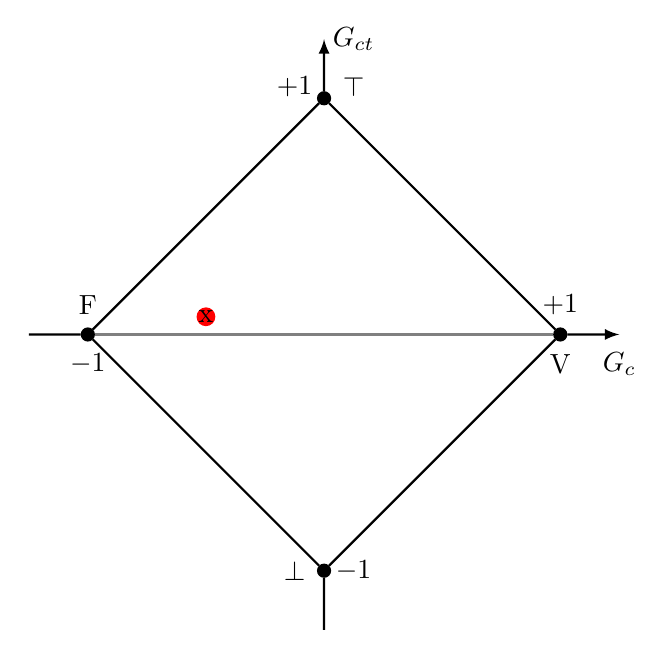
\begin{tikzpicture}[scale=0.75]
\tikzset{ >=latex, inner sep=0pt, outer sep=0pt,  }
%\draw [lightgray, dashed](0,0) grid (10,10);

\node [fill=black, circle] (V) at (9,5) {:};
\node [fill=black, circle] (F) at (1,5) {:};
\node [fill=black, circle] (T) at (5,9) {:};
\node [fill=black, circle] (L) at (5,1) {:};

%\node [fill=black, circle] (N) at (5,7) { };
%\node [fill=black, circle] (S) at (5,3) { };
%\node [fill=black, circle] (E) at (7,5) { };
%\node [fill=black, circle] (W) at (3,5) { };

%\node [fill=black, circle] (NE) at (7,7) { };
%\node [fill=black, circle] (SE) at (7,3) { };
%\node [fill=black, circle] (NW) at (3,7) { };
%\node [fill=black, circle] (SW) at (3,3) { };

%\draw [dashed] (F) -- (V);
%\draw [dashed] (T) -- (L);
\draw [->, thick] (V)   -- (10,5);
\draw [    thick] (0,5) -- (F);
\draw [->, thick] (T)   -- (5,10);
\draw [    thick] (5,0) -- (L);

\draw [thick] (V) -- (T);
\draw [thick] (T) -- (F);
\draw [thick] (F) -- (L);
\draw [thick] (L) -- (V);

%\draw [gray,dashed] (T) -- (L);
\draw [gray,thick] (V) -- (F);
%\draw[thick] (SW) rectangle (NE);
%\fill[nearly transparent] (SW) rectangle (NE);

\node at (10,4.5) {$G_{c}$};
\node at (5.5,10) {$G_{ct}$};

\node at (4.5,9.2) {$+1$};
\node at (9.0,5.5) {$+1$};
\node at (5.5,1.0) {$-1$};
\node at (1.0,4.5) {$-1$};

\node at (9.0,4.5) {V};
\node at (1.0,5.5) {F};
\node at (5.5,9.2) {$\top$};
\node at (4.5,1.0) {$\bot$};

%\node at (5.0,7.0) {\Large{Ligar}};
%\node at (5.0,6.0) {\large{PWM = 100\%}};

%\node at (5.0,3.0) {\Large{Desligar}};
%\node at (5.0,3.0) {\large{PWM = 0\%}};


\node [fill=red, circle] (MU) at (3.0,5.3) {x};

\end{tikzpicture} }
\subfloat[$Gct$ negativo ($\mu_0<\mu_1$)]{\label{fig:gctneg}
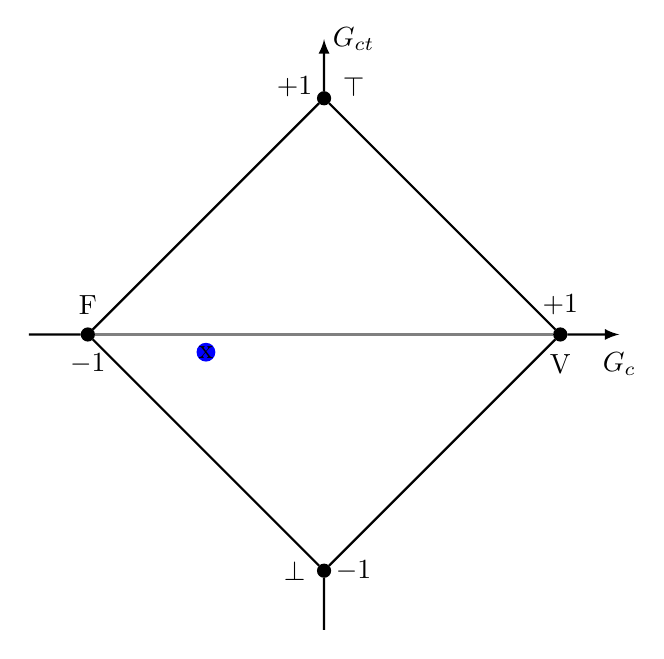
\begin{tikzpicture}[scale=0.75]
\tikzset{ >=latex, inner sep=0pt, outer sep=0pt,  }
%\draw [lightgray, dashed](0,0) grid (10,10);

\node [fill=black, circle] (V) at (9,5) {:};
\node [fill=black, circle] (F) at (1,5) {:};
\node [fill=black, circle] (T) at (5,9) {:};
\node [fill=black, circle] (L) at (5,1) {:};

%\node [fill=black, circle] (N) at (5,7) { };
%\node [fill=black, circle] (S) at (5,3) { };
%\node [fill=black, circle] (E) at (7,5) { };
%\node [fill=black, circle] (W) at (3,5) { };

%\node [fill=black, circle] (NE) at (7,7) { };
%\node [fill=black, circle] (SE) at (7,3) { };
%\node [fill=black, circle] (NW) at (3,7) { };
%\node [fill=black, circle] (SW) at (3,3) { };

%\draw [dashed] (F) -- (V);
%\draw [dashed] (T) -- (L);
\draw [->, thick] (V)   -- (10,5);
\draw [    thick] (0,5) -- (F);
\draw [->, thick] (T)   -- (5,10);
\draw [    thick] (5,0) -- (L);

\draw [thick] (V) -- (T);
\draw [thick] (T) -- (F);
\draw [thick] (F) -- (L);
\draw [thick] (L) -- (V);

%\draw [gray,dashed] (T) -- (L);
\draw [gray,thick] (V) -- (F);
%\draw[thick] (SW) rectangle (NE);
%\fill[nearly transparent] (SW) rectangle (NE);

\node at (10,4.5) {$G_{c}$};
\node at (5.5,10) {$G_{ct}$};

\node at (4.5,9.2) {$+1$};
\node at (9.0,5.5) {$+1$};
\node at (5.5,1.0) {$-1$};
\node at (1.0,4.5) {$-1$};

\node at (9.0,4.5) {V};
\node at (1.0,5.5) {F};
\node at (5.5,9.2) {$\top$};
\node at (4.5,1.0) {$\bot$};

%\node at (5.0,7.0) {\Large{Ligar}};
%\node at (5.0,6.0) {\large{PWM = 100\%}};

%\node at (5.0,3.0) {\Large{Desligar}};
%\node at (5.0,3.0) {\large{PWM = 0\%}};

\node [fill=blue, circle] (MU1) at (3.0,4.7) {x};

\end{tikzpicture}}

\label{fig:sistPrimeiraOrdem}

{\small Fonte: Próprio autor}
\end{figure}



Podemos então notar que 
a diferença existente entre os graus de evidência favoráveis 
é equivalente ao erro, 
como é denominado no sistema clássico de controle, 
mas que na LPA$E\tau$ pode ser considerado como 
o Grau de Contradição, pois,
na condição em que a variável controlada é igual a 
variável de referência, não há erro, e a contradição é zero, 
entretando se a forem diferentes, 
tanto o erro quanto o grau de contradição
serão não nulos. 

A representação do reticulado da LPA$E\tau$ 
para a condição em que o $Gct$ define o estado
de Ligar ou Desligar o sistema é mostrado na 
Figura \ref{fig:reticuladoEtOnOff}.



%%%%%%%%%%%%%%%%%%%%%%%%%%%%%%%%%%%%%%%
%%%%%%%%%%%%%%%%%%%%%%%%%%%%%%%%%%%%%%%



\begin{figure}[!h]
\centering
\caption{Representação do reticulado da LPA$E\tau$ dividido em duas partes}
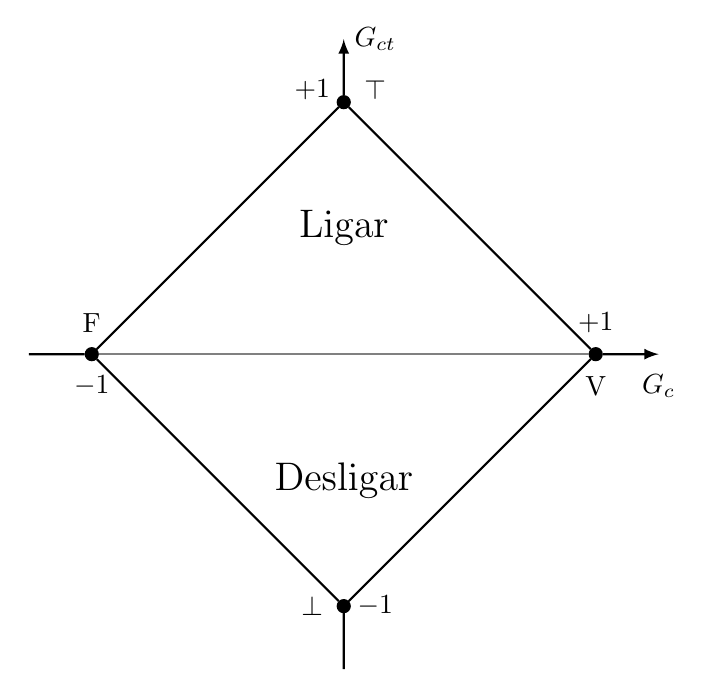
\begin{tikzpicture}[scale=0.8]
\tikzset{ >=latex, inner sep=0pt, outer sep=0pt,  }

%\draw [lightgray, dashed](0,0) grid (10,10);

\node [fill=black, circle] (V) at (9,5) {:};
\node [fill=black, circle] (F) at (1,5) {:};
\node [fill=black, circle] (T) at (5,9) {:};
\node [fill=black, circle] (L) at (5,1) {:};

%\node [fill=black, circle] (N) at (5,7) { };
%\node [fill=black, circle] (S) at (5,3) { };
%\node [fill=black, circle] (E) at (7,5) { };
%\node [fill=black, circle] (W) at (3,5) { };

%\node [fill=black, circle] (NE) at (7,7) { };
%\node [fill=black, circle] (SE) at (7,3) { };
%\node [fill=black, circle] (NW) at (3,7) { };
%\node [fill=black, circle] (SW) at (3,3) { };

%\draw [dashed] (F) -- (V);
%\draw [dashed] (T) -- (L);
\draw [->, thick] (V)   -- (10,5);
\draw [    thick] (0,5) -- (F);
\draw [->, thick] (T)   -- (5,10);
\draw [    thick] (5,0) -- (L);

\draw [thick] (V) -- (T);
\draw [thick] (T) -- (F);
\draw [thick] (F) -- (L);
\draw [thick] (L) -- (V);

%\draw [gray,dashed] (T) -- (L);
\draw [gray,thick] (V) -- (F);
%\draw[thick] (SW) rectangle (NE);
%\fill[nearly transparent] (SW) rectangle (NE);

\node at (10,4.5) {$G_{c}$};
\node at (5.5,10) {$G_{ct}$};

\node at (4.5,9.2) {$+1$};
\node at (9.0,5.5) {$+1$};
\node at (5.5,1.0) {$-1$};
\node at (1.0,4.5) {$-1$};

\node at (9.0,4.5) {V};
\node at (1.0,5.5) {F};
\node at (5.5,9.2) {$\top$};
\node at (4.5,1.0) {$\bot$};

\node at (5.0,7.0) {\Large{Ligar}};
%\node at (5.0,6.0) {\large{PWM = 100\%}};

\node at (5.0,3.0) {\Large{Desligar}};
%\node at (5.0,3.0) {\large{PWM = 0\%}};


\end{tikzpicture}
\label{fig:reticuladoEtOnOff}

{\small Fonte: Próprio autor }
\end{figure}



%%%%%%%%%%%%%%%%%%%%%%%%%%%%%%%%%%%%%%%
%%%%%%%%%%%%%%%%%%%%%%%%%%%%%%%%%%%%%%%


A opção pela ação de controle Liga-Desliga
é interessante do ponto de vista da velocidade 
de resposta ao degrau, 
porém apresenta uma oscilação que, 
a depender da dinâmica do sistema que está sendo trabalhado,
pode gerar uma amplitude maior do que o aceitável,
como pôde ser visto na 
Figura \ref{fig:acaoControleLigaDesliga}.

Outra estratégia simples é a 
utilização do sistema sem realimentação, 
aplicando à saída o valor proporcional desejado.


\section{A variável manipulada}

Para a implementação da saída do bloco 
LPA$E\tau$ de modo equivalente ao sistema em malha aberta,
assumindo não haver contradição, 
e para a Proposição adotada: 
\emph{"P: A velocidade de rotação é máxima"}, 
temos a Reta Perfeitamente Definida como referencial. 

A Figura \ref{fig:gc25} mostra o ponto de operação 
para uma velocidade de 25\% da proposição, 
e a Figura \ref{fig:gc90} mostra o ponto de operação
para a velocidade de 90\% da proposição.

Assim, considerando o Grau de Contradição nulo:

\begin{equation}
Gct = \mu + \lambda - 1 = 0 \rightarrow \mu = 1 - \lambda
\end{equation}

como $\mu_1 = 1 - \lambda$ e $\mu = \mu_0$:

\begin{equation}
\mu_0 = \mu_1
\label{eq:mu0eqmu1}
\end{equation}

substituindo $Gc$ por $\mu-\lambda$ e aplicando $\mu_0$ e $\lambda = 1 - \mu_1$ na Eq. \ref{eq:muer}:

\begin{equation}
\mu_{ER} = \frac{Gc + 1}{2} \rightarrow \mu_{ER} = \frac{(\mu_0 + \mu_2 - 1) + 1}{2} \rightarrow \mu_{ER} = \frac{\mu_0 + \mu_1}{2}
\label{eq:uermu0mu1}
\end{equation}

aplicando \ref{eq:mu0eqmu1} em \ref{eq:uermu0mu1}:

\begin{equation}
\mu_{ER} = \frac{\mu_0 + \mu_0}{2} = \frac{2.\mu_0}{2} = \mu_0
\end{equation}


Assim, adota-se como valor para a variável manipulada 
o valor $\mu_{ER}$, que é o próprio valor do 
grau de evidência favorável ($\mu_0$), 
e pode ser exemplificado na 
Figura \ref{fig:gc25} e na 
Figura \ref{fig:gc90}, 
respectivamente para valores de referência de 25\% e 90\%
do valor máximo da variável controlada, 
que é a velocidade de rotação máxima alcançada 
pelo motor no sistema proposto.






%%%%%%%%%%%%%%%%%%%%%%%%%%%%%%%%%%%%%%%
%%%%%%%%%%%%%%%%%%%%%%%%%%%%%%%%%%%%%%%



\begin{figure}[!htb]
\centering
\caption{Representação do reticulado da LPA$E\tau$}
\subfloat[$Gc = -0,50 \ \ \ \mu_{ER} = 0,25$]{\label{fig:gc25}

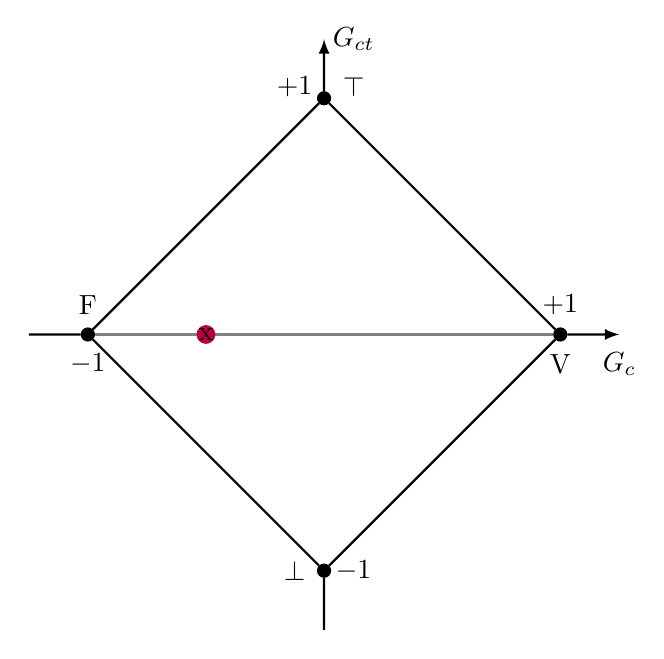
\begin{tikzpicture}[scale=0.75]
\tikzset{ >=latex, inner sep=0pt, outer sep=0pt,  }
%\draw [lightgray, dashed](0,0) grid (10,10);

\node [fill=black, circle] (V) at (9,5) {:};
\node [fill=black, circle] (F) at (1,5) {:};
\node [fill=black, circle] (T) at (5,9) {:};
\node [fill=black, circle] (L) at (5,1) {:};

%\node [fill=black, circle] (N) at (5,7) { };
%\node [fill=black, circle] (S) at (5,3) { };
%\node [fill=black, circle] (E) at (7,5) { };
%\node [fill=black, circle] (W) at (3,5) { };

%\node [fill=black, circle] (NE) at (7,7) { };
%\node [fill=black, circle] (SE) at (7,3) { };
%\node [fill=black, circle] (NW) at (3,7) { };
%\node [fill=black, circle] (SW) at (3,3) { };

%\draw [dashed] (F) -- (V);
%\draw [dashed] (T) -- (L);
\draw [->, thick] (V)   -- (10,5);
\draw [    thick] (0,5) -- (F);
\draw [->, thick] (T)   -- (5,10);
\draw [    thick] (5,0) -- (L);

\draw [thick] (V) -- (T);
\draw [thick] (T) -- (F);
\draw [thick] (F) -- (L);
\draw [thick] (L) -- (V);

%\draw [gray,dashed] (T) -- (L);
\draw [gray,thick] (V) -- (F);
%\draw[thick] (SW) rectangle (NE);
%\fill[nearly transparent] (SW) rectangle (NE);

\node at (10,4.5) {$G_{c}$};
\node at (5.5,10) {$G_{ct}$};

\node at (4.5,9.2) {$+1$};
\node at (9.0,5.5) {$+1$};
\node at (5.5,1.0) {$-1$};
\node at (1.0,4.5) {$-1$};

\node at (9.0,4.5) {V};
\node at (1.0,5.5) {F};
\node at (5.5,9.2) {$\top$};
\node at (4.5,1.0) {$\bot$};

%\node at (5.0,7.0) {\Large{Ligar}};
%\node at (5.0,6.0) {\large{PWM = 100\%}};

%\node at (5.0,3.0) {\Large{Desligar}};
%\node at (5.0,3.0) {\large{PWM = 0\%}};


\node [fill=purple, circle] (MU) at (3.0,5.0) {x};

\end{tikzpicture} }
\subfloat[$Gc = 0,80 \ \ \ \mu_{ER} = 0,90$]{\label{fig:gc90}
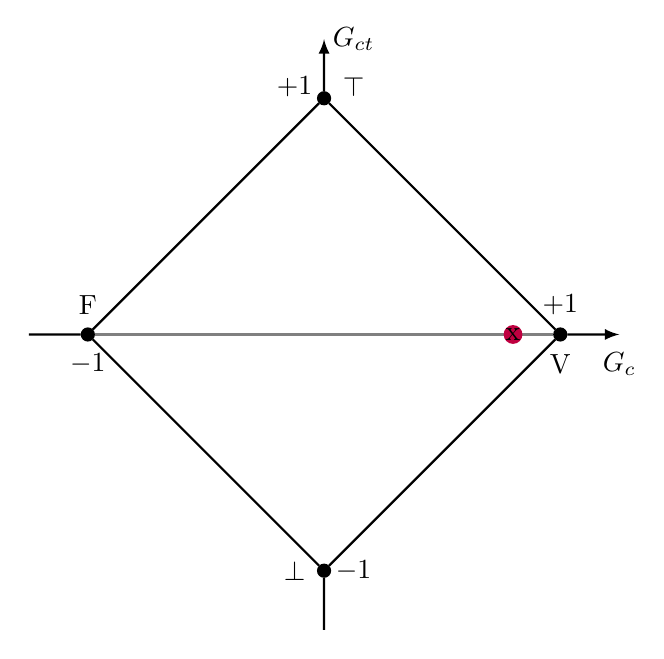
\begin{tikzpicture}[scale=0.75]
\tikzset{ >=latex, inner sep=0pt, outer sep=0pt,  }
%\draw [lightgray, dashed](0,0) grid (10,10);

\node [fill=black, circle] (V) at (9,5) {:};
\node [fill=black, circle] (F) at (1,5) {:};
\node [fill=black, circle] (T) at (5,9) {:};
\node [fill=black, circle] (L) at (5,1) {:};

%\node [fill=black, circle] (N) at (5,7) { };
%\node [fill=black, circle] (S) at (5,3) { };
%\node [fill=black, circle] (E) at (7,5) { };
%\node [fill=black, circle] (W) at (3,5) { };

%\node [fill=black, circle] (NE) at (7,7) { };
%\node [fill=black, circle] (SE) at (7,3) { };
%\node [fill=black, circle] (NW) at (3,7) { };
%\node [fill=black, circle] (SW) at (3,3) { };

%\draw [dashed] (F) -- (V);
%\draw [dashed] (T) -- (L);
\draw [->, thick] (V)   -- (10,5);
\draw [    thick] (0,5) -- (F);
\draw [->, thick] (T)   -- (5,10);
\draw [    thick] (5,0) -- (L);

\draw [thick] (V) -- (T);
\draw [thick] (T) -- (F);
\draw [thick] (F) -- (L);
\draw [thick] (L) -- (V);

%\draw [gray,dashed] (T) -- (L);
\draw [gray,thick] (V) -- (F);
%\draw[thick] (SW) rectangle (NE);
%\fill[nearly transparent] (SW) rectangle (NE);

\node at (10,4.5) {$G_{c}$};
\node at (5.5,10) {$G_{ct}$};

\node at (4.5,9.2) {$+1$};
\node at (9.0,5.5) {$+1$};
\node at (5.5,1.0) {$-1$};
\node at (1.0,4.5) {$-1$};

\node at (9.0,4.5) {V};
\node at (1.0,5.5) {F};
\node at (5.5,9.2) {$\top$};
\node at (4.5,1.0) {$\bot$};

%\node at (5.0,7.0) {\Large{Ligar}};
%\node at (5.0,6.0) {\large{PWM = 100\%}};

%\node at (5.0,3.0) {\Large{Desligar}};
%\node at (5.0,3.0) {\large{PWM = 0\%}};

\node [fill=purple, circle] (MU1) at (8.2,5.0) {x};

\end{tikzpicture}}

\label{fig:sistPrimeiraOrdem}

{\small Fonte: Próprio autor}
\end{figure}


\section{A região de parada}

O sistema possui uma região de operação 
que não é possível realizar o controle, 
pois é a região onde a inércia do sistema parado
impede a movimentação do eixo do motor, 
o que deixa de acontecer em torno dos 10\% do valor do PWM,
de acordo com testes realizados.

Sendo assim, foi definida uma região de para o controlador 
aplicar potência máxima ao sistema, 
e tal região pode ser vista na 
Figura \ref{fig:zonaMorta} e 
denominada como Zona Morta, 
pois para qualquer variação dentro dessa faixa, 
não há variação de velocidade no motor.


\begin{figure}[!h]
\centering
\caption{Representação da zona morta no reticulado da LPA$E\tau$}
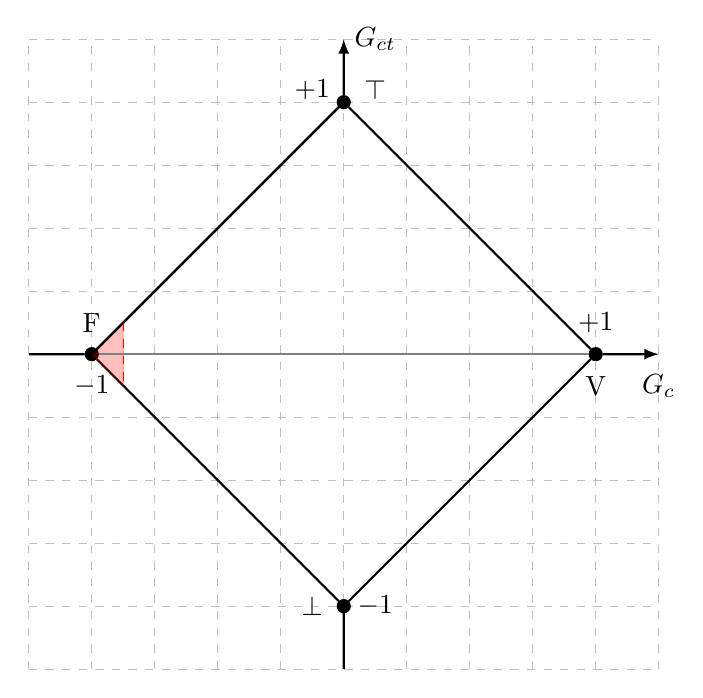
\begin{tikzpicture}[scale=0.80]
\tikzset{ >=latex, inner sep=0pt, outer sep=0pt,  }

\draw [lightgray, dashed](0,0) grid (10,10);

\node [fill=black, circle] (V) at (9,5) {:};
\node [fill=black, circle] (F) at (1,5) {:};
\node [fill=black, circle] (T) at (5,9) {:};
\node [fill=black, circle] (L) at (5,1) {:};

\draw [->, thick] (V)   -- (10,5);
\draw [    thick] (0,5) -- (F);
\draw [->, thick] (T)   -- (5,10);
\draw [    thick] (5,0) -- (L);

\draw [thick] (V) -- (T);
\draw [thick] (T) -- (F);
\draw [thick] (F) -- (L);
\draw [thick] (L) -- (V);

%\draw[thick] (SW) rectangle (NE);
%\fill[nearly transparent] (SW) rectangle (NE);

\node at (10,4.5) {$G_{c}$};
\node at (5.5,10) {$G_{ct}$};

\node at (4.5,9.2) {$+1$};
\node at (9.0,5.5) {$+1$};
\node at (5.5,1.0) {$-1$};
\node at (1.0,4.5) {$-1$};

\node at (9.0,4.5) {V};
\node at (1.0,5.5) {F};
\node at (5.5,9.2) {$\top$};
\node at (4.5,1.0) {$\bot$};

\draw [fill, red,nearly transparent] (1.0,5.0) -- (1.5,5.5) -- (1.5,4.5) -- (1.0,5.0);
\draw [thick] (5.0,9.0) -- (1.0,5.0);
\draw [gray,thick] (V) -- (F);
\draw [dashed, red] (1.5,5.5) -- (1.5,4.5);
\end{tikzpicture}
\label{fig:zonaMorta}

{\small Fonte: Próprio autor }
\end{figure}

A região denominada Zona Morta, 
representa uma região em que o ponto de operação do sistema
estará no momento inicial de partida do sistema, 
em que a variável de referência acabar de ser setada e
a variável controlada ainda estiver na condição nula, 
pelo sistema estar saindo da condição de repouso. 



Outra condição crítica para o sistema é 
quando houver um travamento do eixo do motor,
levando o grau de evidência $\mu_1$ para a condição nula,
ou seja, $\lambda$ para o valor máximo. 
A Figura \ref{fig:travamentoEixo} mostra a região 
que pode sinalizar tal anormalidade.


\begin{figure}[!h]
\centering
\caption{Representação da região de travamento no reticulado da LPA$E\tau$}
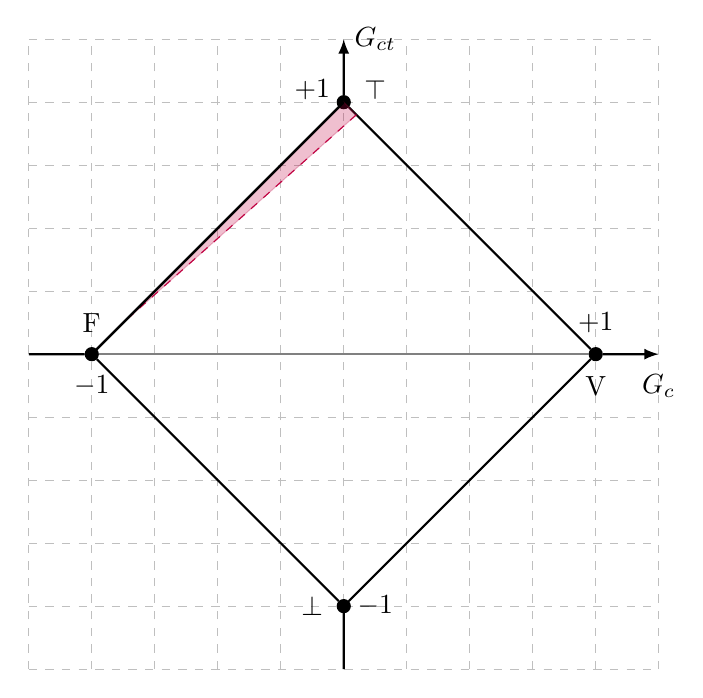
\begin{tikzpicture}[scale=0.80]
\tikzset{ >=latex, inner sep=0pt, outer sep=0pt,  }

\draw [lightgray, dashed](0,0) grid (10,10);

\node [fill=black, circle] (V) at (9,5) {:};
\node [fill=black, circle] (F) at (1,5) {:};
\node [fill=black, circle] (T) at (5,9) {:};
\node [fill=black, circle] (L) at (5,1) {:};

\draw [->, thick] (V)   -- (10,5);
\draw [    thick] (0,5) -- (F);
\draw [->, thick] (T)   -- (5,10);
\draw [    thick] (5,0) -- (L);

\draw [thick] (V) -- (T);
\draw [thick] (T) -- (F);
\draw [thick] (F) -- (L);
\draw [thick] (L) -- (V);

%\draw[thick] (SW) rectangle (NE);
%\fill[nearly transparent] (SW) rectangle (NE);

\node at (10,4.5) {$G_{c}$};
\node at (5.5,10) {$G_{ct}$};

\node at (4.5,9.2) {$+1$};
\node at (9.0,5.5) {$+1$};
\node at (5.5,1.0) {$-1$};
\node at (1.0,4.5) {$-1$};

\node at (9.0,4.5) {V};
\node at (1.0,5.5) {F};
\node at (5.5,9.2) {$\top$};
\node at (4.5,1.0) {$\bot$};


\draw [fill, purple, nearly transparent] (1.5,5.5) -- (5.0,9.0) -- (5.2,8.8) -- (1.5,5.5);
\draw [dashed, purple] (5.2,8.8) -- (1.5,5.5);
\draw [thick] (5.0,9.0) -- (1.0,5.0);
\draw [gray,thick] (V) -- (F);
\end{tikzpicture}
\label{fig:travamentoEixo}

{\small Fonte: Próprio autor }
\end{figure}


Nesta condição o controlador pode tomar a dicisão de 
desligar o sistema controlado, 
levá-lo a condição de falha e 
sinalizar ao operador a irregularidade, 
a depender do tipo de sistema a ser controlado.





\section{ A região de operação }

Para a região de operação, 
foi estipulado e verificado de forma empírica 
um valor de grau de contradição adequado para 
atender os requisitos de desempenho do sistema, 
que foi um grau de contradição contido no 
intervalo $[-0,1;0,1]$. 



\begin{figure}[!h]
\centering
\caption{Representação da região ativa no reticulado da LPA$E\tau$}
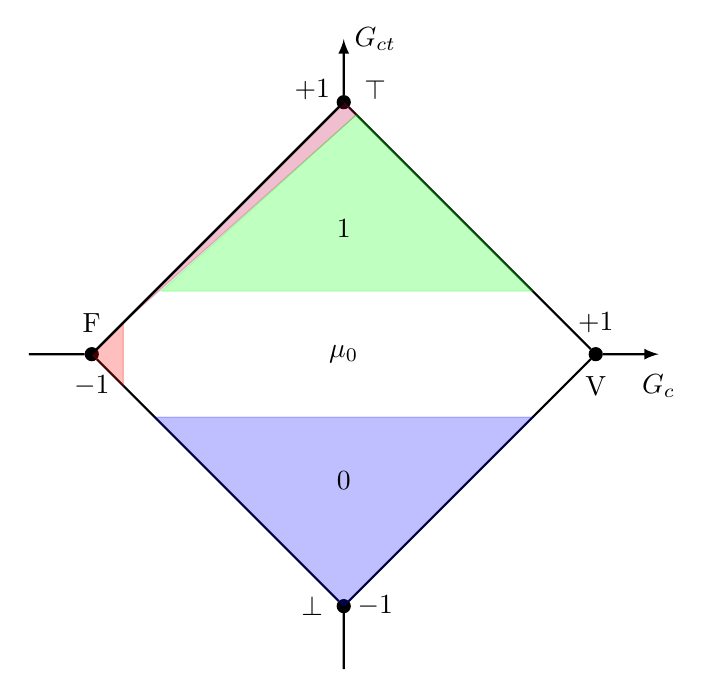
\begin{tikzpicture}[scale=0.80]
\tikzset{ >=latex, inner sep=0pt, outer sep=0pt,  }

%\draw [lightgray, dashed](0,0) grid (10,10);

\node [fill=black, circle] (V) at (9,5) {:};
\node [fill=black, circle] (F) at (1,5) {:};
\node [fill=black, circle] (T) at (5,9) {:};
\node [fill=black, circle] (L) at (5,1) {:};

\draw [->, thick] (V)   -- (10,5);
\draw [    thick] (0,5) -- (F);
\draw [->, thick] (T)   -- (5,10);
\draw [    thick] (5,0) -- (L);

\draw [thick] (V) -- (T);
\draw [thick] (T) -- (F);
\draw [thick] (F) -- (L);
\draw [thick] (L) -- (V);

%\draw[thick] (SW) rectangle (NE);
%\fill[nearly transparent] (SW) rectangle (NE);

\node at (10,4.5) {$G_{c}$};
\node at (5.5,10) {$G_{ct}$};

\node at (4.5,9.2) {$+1$};
\node at (9.0,5.5) {$+1$};
\node at (5.5,1.0) {$-1$};
\node at (1.0,4.5) {$-1$};

\node at (9.0,4.5) {V};
\node at (1.0,5.5) {F};
\node at (5.5,9.2) {$\top$};
\node at (4.5,1.0) {$\bot$};

\draw [fill, red,nearly transparent] (1.0,5.0) -- (1.5,5.5) -- (1.5,4.5) -- (1.0,5.0);
\draw [fill, purple, nearly transparent] (1.5,5.5) -- (5.0,9.0) -- (5.2,8.8) -- (1.5,5.5);
\draw [fill, blue, nearly transparent] (5.0,1.0) -- (8.0,4.0) -- (2.0,4.0) -- (5.0,1.0);
\draw [fill, green, nearly transparent] (5.2,8.8) -- (2.1,6.0) -- (8.0,6.0) -- (5.2,8.8);


%\draw [dashed, purple] (5.2,8.8) -- (1.5,5.5);
\draw [thick] (5.0,9.0) -- (1.0,5.0);
%\draw [gray,thick] (V) -- (F);


\node at (5.0,7.0) {1};
\node at (5.0,5.0) {$\mu_0$};
\node at (5.0,3.0) {0};

\end{tikzpicture}
\label{fig:regiaoAtiva}

{\small Fonte: Próprio autor }
\end{figure}




Os valores de $Gct > 0,1$ geram na saída o valor máximo,
1,0. Na região oposta, para $Gct < -0,1$ a saída assume
 o valor nulo, 0. 

Aplicando um degrau à entrada do sistema, 
podemos perceber o gráfico da 
Figura \ref{fig:acaoLPAEtgct100} 
que o tempo de acomodação é reduzido drasticamente, 
apesar do sobressinal gerado, 
este não apresenta problema por estar 
dentro da tolerância aceitável. 


\begin{figure}[!htb]
\caption{Ação de controle utilizando LPA$E\tau$}
\vspace{-1cm}\center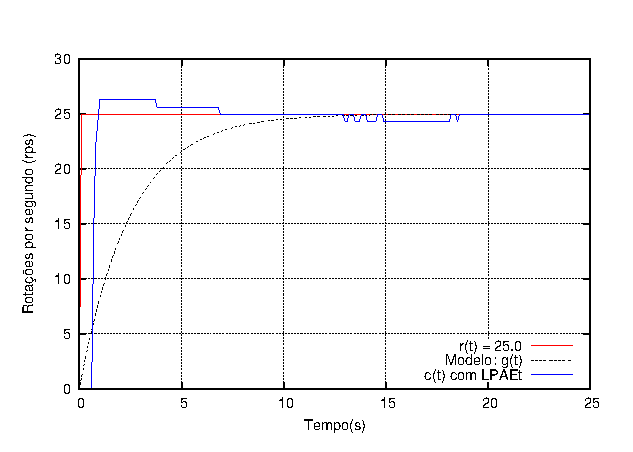
\includegraphics[scale=1.6]{./imagens/LPAEt-gct100.eps}
\label{fig:acaoLPAEtgct100}

{\small Fonte: Próprio autor}
\end{figure}

Como a relação entre o valor de referência e a 
velocidade de rotação do motor não é perfeitamente linear,
para cada valor de patamar pode haver um erro considerável,
inclusive sendo maior do que o valor permitido pela 
tolerância. 

Assim para reduzir o grau de contradição
em decorrência dessa não linearidade, 
é somado ao $\mu_0$ um valor de correção denominado $\delta$.

Então a representação do reticulado da LPA$E\tau$ 
fica da seguinte forma mostrada na 
Figura \ref{fig:regiaoAtivaMuDelta}. 


\begin{figure}[!h]
\centering
\caption{Representação da região ativa no reticulado da LPA$E\tau$}
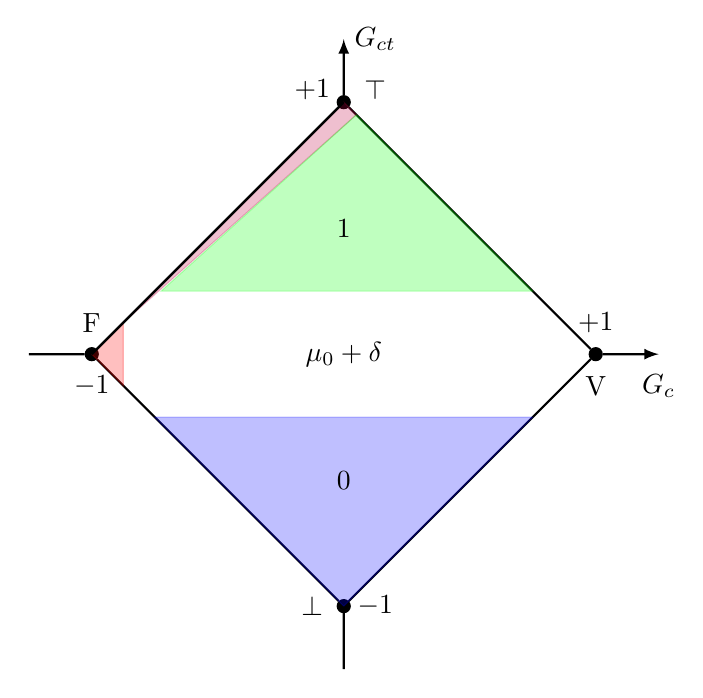
\begin{tikzpicture}[scale=0.80]
\tikzset{ >=latex, inner sep=0pt, outer sep=0pt,  }

%\draw [lightgray, dashed](0,0) grid (10,10);

\node [fill=black, circle] (V) at (9,5) {:};
\node [fill=black, circle] (F) at (1,5) {:};
\node [fill=black, circle] (T) at (5,9) {:};
\node [fill=black, circle] (L) at (5,1) {:};

\draw [->, thick] (V)   -- (10,5);
\draw [    thick] (0,5) -- (F);
\draw [->, thick] (T)   -- (5,10);
\draw [    thick] (5,0) -- (L);

\draw [thick] (V) -- (T);
\draw [thick] (T) -- (F);
\draw [thick] (F) -- (L);
\draw [thick] (L) -- (V);

%\draw[thick] (SW) rectangle (NE);
%\fill[nearly transparent] (SW) rectangle (NE);

\node at (10,4.5) {$G_{c}$};
\node at (5.5,10) {$G_{ct}$};

\node at (4.5,9.2) {$+1$};
\node at (9.0,5.5) {$+1$};
\node at (5.5,1.0) {$-1$};
\node at (1.0,4.5) {$-1$};

\node at (9.0,4.5) {V};
\node at (1.0,5.5) {F};
\node at (5.5,9.2) {$\top$};
\node at (4.5,1.0) {$\bot$};

\draw [fill, red,nearly transparent] (1.0,5.0) -- (1.5,5.5) -- (1.5,4.5) -- (1.0,5.0);
\draw [fill, purple, nearly transparent] (1.5,5.5) -- (5.0,9.0) -- (5.2,8.8) -- (1.5,5.5);
\draw [fill, blue, nearly transparent] (5.0,1.0) -- (8.0,4.0) -- (2.0,4.0) -- (5.0,1.0);
\draw [fill, green, nearly transparent] (5.2,8.8) -- (2.1,6.0) -- (8.0,6.0) -- (5.2,8.8);


%\draw [dashed, purple] (5.2,8.8) -- (1.5,5.5);
\draw [thick] (5.0,9.0) -- (1.0,5.0);
%\draw [gray,thick] (V) -- (F);


\node at (5.0,7.0) {1};
\node at (5.0,5.0) {$\mu_0 + \delta$};
\node at (5.0,3.0) {0};

\end{tikzpicture}
\label{fig:regiaoAtivaMuDelta}

{\small Fonte: Próprio autor }
\end{figure}



A região ativa então pode ser dividida em 
tantas partes quantas forem necessárias 
para garantir um $\delta$ satisfatório para tal região,
pois tal valor não garante erro nulo para toda extensão
possível.





%######################################
\begin{comment}


\begin{figure}[!h]
\centering
\caption{Representação da região ativa no reticulado da LPA$E\tau$}
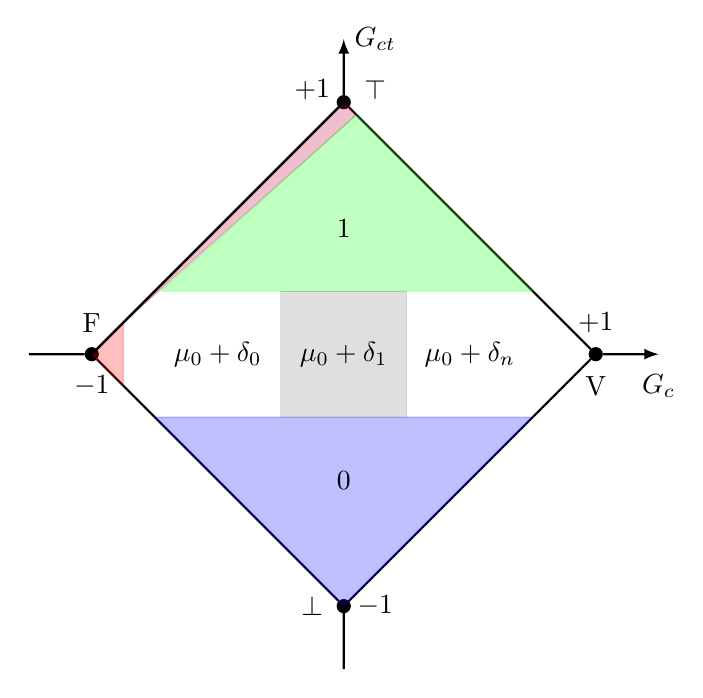
\begin{tikzpicture}[scale=0.80]
\tikzset{ >=latex, inner sep=0pt, outer sep=0pt,  }

%\draw [lightgray, dashed](0,0) grid (10,10);

\node [fill=black, circle] (V) at (9,5) {:};
\node [fill=black, circle] (F) at (1,5) {:};
\node [fill=black, circle] (T) at (5,9) {:};
\node [fill=black, circle] (L) at (5,1) {:};

\draw [->, thick] (V)   -- (10,5);
\draw [    thick] (0,5) -- (F);
\draw [->, thick] (T)   -- (5,10);
\draw [    thick] (5,0) -- (L);

\draw [thick] (V) -- (T);
\draw [thick] (T) -- (F);
\draw [thick] (F) -- (L);
\draw [thick] (L) -- (V);

%\draw[thick] (SW) rectangle (NE);
%\fill[nearly transparent] (SW) rectangle (NE);

\node at (10,4.5) {$G_{c}$};
\node at (5.5,10) {$G_{ct}$};

\node at (4.5,9.2) {$+1$};
\node at (9.0,5.5) {$+1$};
\node at (5.5,1.0) {$-1$};
\node at (1.0,4.5) {$-1$};

\node at (9.0,4.5) {V};
\node at (1.0,5.5) {F};
\node at (5.5,9.2) {$\top$};
\node at (4.5,1.0) {$\bot$};

\draw [fill, red,nearly transparent] (1.0,5.0) -- (1.5,5.5) -- (1.5,4.5) -- (1.0,5.0);
\draw [fill, purple, nearly transparent] (1.5,5.5) -- (5.0,9.0) -- (5.2,8.8) -- (1.5,5.5);
\draw [fill, blue, nearly transparent] (5.0,1.0) -- (8.0,4.0) -- (2.0,4.0) -- (5.0,1.0);
\draw [fill, green, nearly transparent] (5.2,8.8) -- (2.1,6.0) -- (8.0,6.0) -- (5.2,8.8);

\draw [fill, gray, nearly transparent] (4.0,6.0) -- (4.0,4.0)-- (6.0,4.0) -- (6.0,6.0) -- (4.0,6.0);


%\draw [dashed, purple] (5.2,8.8) -- (1.5,5.5);
\draw [thick] (5.0,9.0) -- (1.0,5.0);
%\draw [gray,thick] (V) -- (F);


\node at (5.0,7.0) {1};
\node at (3.0,5.0) {$\mu_0 + \delta_0$};
\node at (5.0,5.0) {$\mu_0 + \delta_1$};
\node at (7.0,5.0) {$\mu_0 + \delta_n$};
\node at (5.0,3.0) {0};

\end{tikzpicture}
\label{fig:regiaoAtivaMuDeltaN}

{\small Fonte: Próprio autor }
\end{figure}


\end{comment}
%######################################



Para gerar um divisão de valores alvo, 
em que o erro seja de no máximo 5\%, 
foi gerada uma tabela que tem como valor inicial
o 10, pois é assumido que para o sistema em estudo,
valores abaixo são considerados zona morta.

A cada incremento de 10\% aproximadamente, 
é gerado o próximo elemento, até o máximo valor menor do que
100, equivalente à 100\% do valor máximo de saída.

Sendo assim segue a 
Tabela \ref{tab:correcaoDelta} 
com os respectivos valores alvo, 
os limites inferiores e superiores, 
que são calculados baseados em decremento de 5\% e
incremento de 5\%, respectivamente, ao valor alvo.

Para todo valor alvo, uma variação positiva ou negativa
de 5\% está enquadrada dentro dos limites motrados na Tabela.

Esses intervalos abrangem todo o intervalo entre 
o valor 10 e o 100, mínimo e máximo, 
de modo a qualquer valor desejado fique 
dentro de algum intervalo, 
e possua um valor alvo bem próximo.


\begin{table}[h]
\centering
\caption{Valores de correção para a condição de contradição}
\label{tab:correcaoDelta}

\begin{tabular}{c|c|c||c}
\hline
%Intervalo de amostras  &  erro médio relativo \\ \hline
Limite Inferior & Alvo & Limite Superior & Valor de Correção\\ \hline
\hline
%0 a 1 $\tau$ & 83,40 \% \\ \hline
10,0 & 10 & 10,7 & $\delta_0$ \\ \hline
10,7 & 11 & 11,7 & $\delta_1$ \\ \hline
11,7 & 12 & 12,8 & $\delta_2$ \\ \hline
12,8 & 13 & 14,3 & $\delta_3$ \\ \hline
14,3 & 15 & 15,8 & $\delta_4$ \\ \hline
15,8 & 16 & 17,3 & $\delta_5$ \\ \hline
17,3 & 18 & 19,4 & $\delta_6$ \\ \hline
19,4 & 20 & 21,4 & $\delta_7$ \\ \hline
21,4 & 22 & 23,5 & $\delta_8$ \\ \hline
23,5 & 24 & 26,0 & $\delta_9$ \\ \hline
26,0 & 27 & 29,1 & $\delta_{10}$ \\ \hline
29,1 & 30 & 32,2 & $\delta_{11}$ \\ \hline
32,2 & 33 & 35,2 & $\delta_{12}$ \\ \hline
35,2 & 36 & 38,3 & $\delta_{13}$ \\ \hline
38,3 & 39 & 41,9 & $\delta_{14}$ \\ \hline
41,9 & 43 & 46,0 & $\delta_{15}$ \\ \hline
46,0 & 47 & 50,0 & $\delta_{16}$ \\ \hline
50,0 & 51 & 54,6 & $\delta_{17}$ \\ \hline
54,6 & 56 & 60,2 & $\delta_{18}$ \\ \hline
60,2 & 62 & 66,4 & $\delta_{19}$ \\ \hline
66,4 & 68 & 73,0 & $\delta_{20}$ \\ \hline
73,0 & 75 & 80,2 & $\delta_{21}$ \\ \hline
80,2 & 82 & 88,3 & $\delta_{22}$ \\ \hline
88,3 & 91 &100,0 & $\delta_{23}$ \\ \hline

\end{tabular}

{\vspace{0.2cm} \small Fonte: Próprio autor}
\end{table}


Para cada valor alvo, há um valor $\delta$ associado, 
que é um valor de correção.
Tomando como exemplo o valor de referência 25\%, 
no momento inicial o vai haver uma grande contradição,
então o reticulado vai ter como saída o valor 1, 
do estado de valor máximo apresentado na 
Figura \ref{fig:regiaoAtivaMuDelta}.

O sistema então está com potência máxima, 
vencendo a inércia do sistema que estava em repouso.
O grau de contradição é reduzido conforme 
o sistema se aproxiima do ponto de operação desejado,
e quando o seu valor é menor do que 
o parâmetro de limite, nesse caso estabelecido em 0,10,
a saída assume o valor equivalente ao $\mu_0$, ou seja,
o valor de referência, então: $\mu_0 = 0,25$, porém 
é acrescido o valor do $\delta_9$, 
que refere-se ao intervalo em que se encontra o 25\%.

Assim a saída do controlador LPA$E\tau$ é 
$\mu_0 + \delta_9$
para um valor de referência de 25\% do valor máximo.











\section{O fator de correção $\delta$}

Um temporizador é implementado de modo a 
gerar um primeiro intevalo de 3 segundos para 
partida e acomodação do sistema, 
em seguida a cada 1 segundo é feita uma verificação
do grau de contradição, 
e como resultado dessa verificação, 
um incremento do fator de correção $\delta$ 
que está em operação é realizada. 

Assim, de forma adaptativa, 
os valores de $\delta$ sempre estão sendo atualizados
para variações que possam ocorrer no processo. 

Caso o tempo de 1 segundo seja muito alto para um 
determinado processo, 
para as perturbações envolvidas no processo,
o tempo pode ser alterado para gerar uma resposta 
mais rápida ou mais lenta. 


















%!@#
%%%%%%%%%%%%%%%%%%%%%%%%%%%%%%%%%%%%%%%
%%%%%%%%%%%%%%%%%%%%%%%%%%%%%%%%%%%%%%%

\newpage


\section{Resultados}


%%%%%%%%%%%%%%%%%%%%%%%%%%%%%%%%%%%%%%%%%%%%%%%%%%
%%%%%%%%%%%%%%%%%%%%%%%%%%%%%%%%%%%%%%%%%%%%%%%%%%
%%%%%%%%%%%%%%%%%%%%%%%%%%%%%%%%%%%%%%%%%%%%%%%%%%
%%%%%%%%%%%%%%%%%%%%%%%%%%%%%%%%%%%%%%%%%%%%%%%%%%




\section{Etapas a serem desenvolvidas}

\begin{itemize}
\item Estudar a LPA2v;
\item Implementar um controlador utilizando LPA2v;
	\begin{itemize}
	\item Estabelecer a configuração do sistema;
	\item Descrever o controlador e parâmetros de ajuste;
	\end{itemize}
\item Otimizar parâmetros e analisar performance;
\end{itemize}


